
\documentclass[]{mcdowellcv}

% ---------- Packages ----------
\usepackage[utf8]{inputenc}
\usepackage{graphicx}
\usepackage{amsmath}
\usepackage[HTML]{xcolor}
\usepackage{hyperref}
\usepackage{csquotes}
\usepackage{multicol}

% ---------- Colors & Links ----------
\definecolor{mygreen}{HTML}{427B58}
\hypersetup{
  colorlinks   = true,
  linkcolor    = purple,
  urlcolor     = purple,
  citecolor    = gray
}

% Little “linky” arrow for visual affordance
\newcommand{\linkarrow}{\,\raisebox{0.15ex}{\footnotesize$\nearrow$}} % ↗

% ---------- Header ----------
\name{aayush bajaj\linebreak {\scriptsize AI/ML Engineer \;·\; Computer Scientist}}
\address{
  \href{mailto:j@abaj.ai}{\raisebox{-2pt}{
\includegraphics[width=0.4cm]{img/mail.png}}: j@abaj.ai\linkarrow} \linebreak
  \href{tel:+61481910408}{\raisebox{-2pt}{
\includegraphics[width=0.4cm]{img/tel.png}}: (+61) 481 910 408}
}
\contacts{
  \href{https://github.com/abaj8494}{\raisebox{-2pt}{
\includegraphics[width=0.4cm]{img/github.png}}: abaj8494\linkarrow} \linebreak
  \href{https://www.linkedin.com/in/aayush-bajaj-b655231a6}{\raisebox{-2pt}{
\includegraphics[width=0.4cm]{img/linkedin.png}}: Aayush Bajaj\linkarrow}
}

\begin{document}
\setcounter{footnote}{0}
\renewcommand{\thefootnote}{\fnsymbol{footnote}}
\footnotetext{\hfill * references and transcript available upon request}
\makeheader

% ---------- SUMMARY ----------
\begin{cvsection}{Summary}
  \begin{cvsubsection}{}{}{}
      Early-career AI/ML engineer (B.CompSci, AI stream) skilled at building \textbf{end-to-end ML systems}: data prep, model training and evaluation in Jupyter; productionising with modern tooling (APIs, containers, CI/CD). Clear docs, small demos, and measurable results. Correspondingly interested in the theoretical Mathematics and Statistics of ML -- grad school deferred.
  \end{cvsubsection}
\end{cvsection}

\vspace{-0.3cm}
% ---------- SKILLS ----------
\begin{cvsection}{Skills}
  \begin{cvsubsection}{}{}{}
    \begin{itemize}
      \item \textbf{Languages:} Python, TypeScript/JavaScript, Java, C, Go, SQL, Lisp
      \item \textbf{ML \& Data:} PyTorch, scikit-learn, NumPy, Pandas, OpenCV, Jupyter, PostgreSQL
      \item \textbf{Systems/Tools:} Linux (bash, vim, tmux, ssh, emacs), Git/GitHub, \LaTeX{}, Docker, Kubernetes, CI/CD
      \item \textbf{Focus:} Computer Vision, Retrieval/RAG, Reproducible ML, Evaluation \& Experimentation, Ethical AI
    \end{itemize}
  \end{cvsubsection}
\end{cvsection}

\vspace{-0.1cm}
% ---------- PROJECTS ----------
\begin{cvsection}{Projects}
  \begin{cvsubsection}{}{}{}

    \begin{itemize}
      \item \textbf{Kidney Segmentation (KiTS19)} —
            \href{https://kits19.grand-challenge.org/evaluation/965bcad2-cbb9-42a8-8b56-a777c9f165e2/}{Leaderboard \#57\linkarrow}
            \hfill \emph{\small nnU-Net, Python, CV, HPC}
            \begin{itemize}
              \item Reproduced nnU-Net end-to-end: data preprocessing, 5-fold training, validation and inference.
              \item Tuned augmentations and inference settings; packaged artifacts for straightforward reproduction.
              \item Wrote a concise technical write-up linking code, configuration, and results.
            \end{itemize}

      \item \textbf{\href{https://bots.abaj.ai}{Bookbot\linkarrow}} — Conversational Q\&A over classic books
            \hfill \emph{\small React/TS, Node/Express, PostgreSQL(pgvector)}
            \begin{itemize}
              \item Auth (OAuth2/JWT), vector search with embeddings, persistent block storage + caching.
              \item Web app with book grid, SVG covers, live processing status; usage caps and Stripe tiering.
            \end{itemize}

      \item \textbf{\href{https://tools.abaj.ai}{Mathematical Tools\linkarrow}} — 23 calculators \& converters
            \hfill \emph{\small Go API, Vanilla JS, Nginx, systemd, HTTPS}
            \begin{itemize}
              \item Compact Go REST API powering number theory, combinatorics, stats, base/temperature, algebra, and linear algebra tools.
              \item Static frontend with responsive grid; deployed behind Nginx with a systemd service.
            \end{itemize}

      \item \textbf{\href{https://github.com/abaj8494/bytelocker}{Bytelocker\linkarrow}} — Neovim plugin for quick file/snippet encryption
            \hfill \emph{\small Lua}
            \begin{itemize}
              \item Designed a lightweight workflow to encrypt/decrypt buffers or regions without leaving the editor.
              \item Added sensible defaults, commands and README examples to encourage adoption. Cross-posted on Reddit / LinkedIn.
            \end{itemize}

      \item \textbf{\href{https://abaj.ai}{Personal Website\linkarrow}} — Notes, demos and write-ups
            \hfill \emph{\small Python, MathJax, Emacs}
            \begin{itemize}
              \item Publishes technical essays, project pages and interactive snippets; keeps documentation close to code.
            \end{itemize}

      \item \textbf{10,000 Hours of Machine Learning} —
            \href{https://github.com/abaj8494/10khrs-ai-ml-dl}{Monorepo\linkarrow}
            \hfill \emph{\small Jupyter}
            \begin{itemize}
              \item A set of self-contained notebooks covering the drosophila of AI, ML, DL, CV and NLP. Experiments and interview problems version controlled too.
            \end{itemize}

      \item \textbf{Selected mini-sites:}
            \href{https://abaj.ai/projects/csp/train-game/}{Sydney Train Game Solver\linkarrow},\;
            \href{https://abaj8494.github.io/shrine/}{Shrine\linkarrow},\;
            \href{https://abaj8494.github.io/gol/}{Game of Life\linkarrow},\;
            \hfill \emph{\small Python, JavaScript}
    \end{itemize}

  \end{cvsubsection}
\end{cvsection}

\vspace{-0.2cm}
% ---------- EDUCATION ----------
\begin{cvsection}{Education}
  \begin{cvsubsection}{B.Science (Artificial Intelligence)}{University of New South Wales}{2021–2025}
    \begin{multicols}{3}
      \begin{itemize}
        \item \small AI stream; Mathematics minor
      \end{itemize}
      \centering{
\includegraphics[width=0.5cm]{img/unsw.png}}
      \flushright{\small Sydney, Australia}
    \end{multicols}
    \vspace{-0.5em}
  \end{cvsubsection}
\end{cvsection}

\vspace{-0.4cm}
% ---------- EXPERIENCE ----------
\begin{cvsection}{Experience}
  \begin{cvsubsection}{Tutor (Private)}{Self-employed}{2019–2023}
    \begin{itemize}
      \item Coached high-school students in mathematics and English; structured weekly drills and feedback to improve grades from C/D toward B/A range.
    \end{itemize}
  \end{cvsubsection}

  \begin{cvsubsection}{Presenter}{Connect Education}{2022}
    \begin{itemize}
      \item Built and delivered intensive “crash-course” seminars in mathematics and English to HSC cohorts.
    \end{itemize}
  \end{cvsubsection}

  \begin{cvsubsection}{Classroom Tutor}{XCD Education}{2020–2021}
    \begin{itemize}
      \item Produced and marked HSC English materials at scale; collaborated with staff on delivery timelines.
    \end{itemize}
  \end{cvsubsection}
\end{cvsection}

% ---------- PORTFOLIO ----------
\begin{cvsection}{Portfolio \& Code}
  \begin{cvsubsection}{}{}{}
    \begin{itemize}
      \item \href{https://abaj.ai}{\raisebox{-2pt}{
\includegraphics[width=0.4cm]{img/abaj.png}}\,abaj.ai\linkarrow}
            \;|\;
            \href{https://github.com/abaj8494}{\raisebox{-2pt}{
\includegraphics[width=0.4cm]{img/github.png}}\,github.com/abaj8494\linkarrow}
            \;|\;
            \href{https://bots.abaj.ai}{\raisebox{-2pt}{
\includegraphics[width=0.4cm]{img/bookbot.png}}\,bots.abaj.ai\linkarrow}
            \;|\;
            \href{https://tools.abaj.ai}{\raisebox{-2pt}{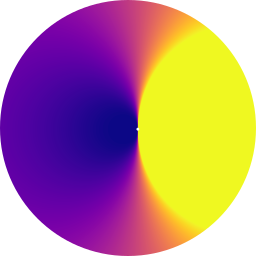
\includegraphics[width=0.4cm]{img/tools.png}}\,tools.abaj.ai\linkarrow}
    \end{itemize}
  \end{cvsubsection}
\end{cvsection}

% (References available upon request.)
\end{document}
